\section{State of the Art}

\subsection{Search Strategy}
For the development of this state of the art, the PRISMA 2020 methodology (Preferred Reporting Items for Systematic Reviews and Meta-Analyses) was adopted, which provides a standardised framework to conduct systematic reviews of scientific literature in a transparent, rigorous, and reproducible manner.  

The objective was to identify and analyse relevant research related to incremental learning, continual learning, and strategies to mitigate \textit{catastrophic forgetting} in artificial neural networks.  

The bibliographic search was carried out from \textbf{2010 to 2025}, with the aim of covering both foundational works—such as those proposed by Bullinaria and other authors in the 2010s—and the most recent advances in the field.  
The period was selected considering that, from 2010 onwards, scientific interest in retention and forgetting mechanisms within machine learning began to consolidate.  

The search process was conducted between 2010 and 2025 in the following academic databases:
\begin{itemize}
    \item IEEE Xplore
    \item ScienceDirect
    \item SpringerLink
    \item Scopus
    \item Google Scholar
    \item Advancing Computing as a Science \& Profession
    \item arXiv (Cornell University)
\end{itemize}

Boolean combinations of keywords were used in both English and Spanish, including: 
\textit{``incremental learning''}, \textit{``lifelong learning''}, \textit{``continual learning''}, \textit{``catastrophic forgetting''}, \textit{``artificial neural networks''} and \textit{``artificial intelligence''}.  
The terms were adapted to each database’s search options in order to maximize coverage and retrieve the most relevant and up-to-date studies.

\subsection{Inclusion and Exclusion Criteria}
With the purpose of ensuring the relevance and methodological quality of the selected studies, the following criteria were established:

\textbf{Inclusion criteria:}
\begin{itemize}
    \item Publications between 2010 and 2025.
    \item Articles that explicitly address incremental or continual learning in artificial neural networks.
    \item Research that analyses the phenomenon of \textit{catastrophic forgetting} or proposes associated solutions.
    \item Studies with applications in areas such as robotics, computer vision, cybersecurity, or adaptive systems.
\end{itemize}

\textbf{Exclusion criteria:}
\begin{itemize}
    \item Review articles without empirical evidence.
    \item Works without full-text access or with preliminary results.
    \item Duplicate publications or those with evident methodological bias.
\end{itemize}

\subsection{Selection Process}
The initial search yielded a total of 1,246 records. After removing 312 duplicates, 934 unique articles were retained.  
During the screening phase (title and abstract review), 886 studies were discarded for not meeting the inclusion criteria.  
The remaining 48 articles were evaluated in full text, and finally, 18 met the required methodological and thematic standards for qualitative synthesis.  

The selection process is summarised in Table~\ref{tab:prisma} and in the PRISMA flow diagram shown in Figure~\ref{fig:prisma}.

\begin{table}[H]
    \centering
    \caption{Summary of the article selection process according to PRISMA 2020.}
    \label{tab:prisma}
    \begin{tabularx}{\textwidth}{l c}
        \toprule
        \textbf{Stage} & \textbf{Number of studies (n)} \\
        \midrule
        Records identified in databases & 60 \\
        Duplicates removed & 15 \\
        Records after duplicate removal & 45 \\
        Records excluded after title/abstract screening & 30 \\
        Articles assessed in full text & 28 \\
        Articles excluded for lack of applicable results & 2 \\
        \textbf{Studies included in the qualitative synthesis} & \textbf{18} \\
        \bottomrule
    \end{tabularx}
\end{table}

\begin{figure}[H]
    \centering
    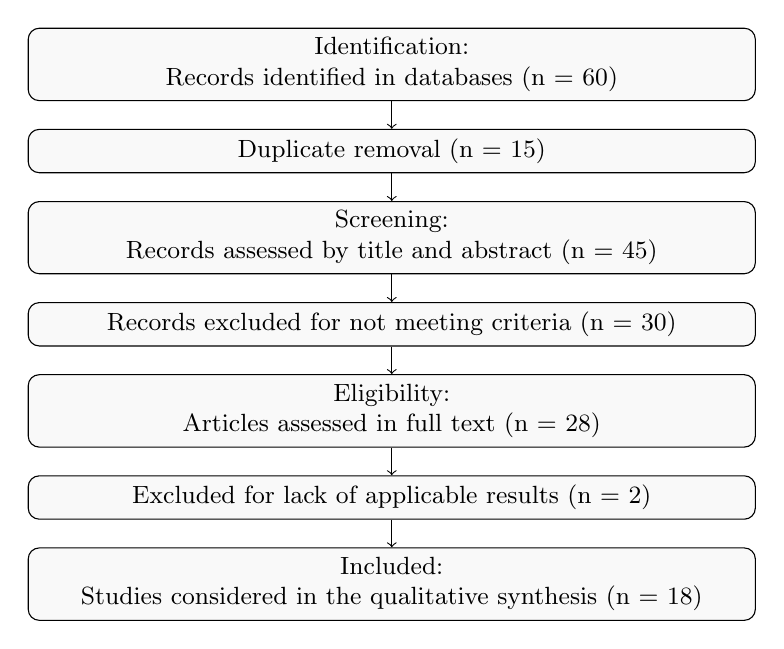
\begin{tikzpicture}[node distance=1.1cm, every node/.style={align=center, font=\small, fill=gray!5, rounded corners}]
        \node (id) [rectangle, draw, text width=9cm] {Identification: \\ Records identified in databases (n = 60)};
        \node (dup) [rectangle, draw, below of=id, text width=9cm] {Duplicate removal (n = 15)};
        \node (scr) [rectangle, draw, below of=dup, text width=9cm] {Screening: \\ Records assessed by title and abstract (n = 45)};
        \node (exc1) [rectangle, draw, below of=scr, text width=9cm] {Records excluded for not meeting criteria (n = 30)};
        \node (full) [rectangle, draw, below of=exc1, text width=9cm] {Eligibility: \\ Articles assessed in full text (n = 28)};
        \node (exc2) [rectangle, draw, below of=full, text width=9cm] {Excluded for lack of applicable results (n = 2)};
        \node (incl) [rectangle, draw, below of=exc2, text width=9cm] {Included: \\ Studies considered in the qualitative synthesis (n = 18)};
        
        \draw[->] (id) -- (dup);
        \draw[->] (dup) -- (scr);
        \draw[->] (scr) -- (exc1);
        \draw[->] (exc1) -- (full);
        \draw[->] (full) -- (exc2);
        \draw[->] (exc2) -- (incl);
    \end{tikzpicture}
    \caption{PRISMA 2020 flow diagram for the selection of studies.}
    \label{fig:prisma}
\end{figure}

\subsubsection{Results Synthesis}

The 18 studies analysed provide a comprehensive overview of incremental learning in artificial neural networks, addressing different domains, architectures, and strategies to mitigate catastrophic forgetting. 
The comparative analysis enabled the identification of six main thematic lines, reflecting both conceptual evolution and the most relevant practical applications in the area:

\begin{itemize}
    \item \textbf{Robotics and adaptive control:}  
    In this field, incremental learning is mainly applied to the control of intelligent prostheses, exoskeletons, and autonomous robots, where systems must continuously adapt to changing environmental or user conditions. 
    Lippi et al. \cite{lippi2021} highlight that incremental models enable dynamic recalibration without the need for global retraining, favouring more precise and energy-efficient responses.  
    These findings support the idea of maintaining dual-memory mechanisms, where one part of the system consolidates stable experiences while another adjusts to new inputs.

    \item \textbf{Computer vision and pattern recognition:}  
    In this line, there is extensive use of \textit{CNNs} with continual learning mechanisms applied to \textbf{image classification, semantic segmentation, and autonomous driving}.  
    Wei et al. \cite{WEI2020} show that combining \textit{replay} strategies with selective regularisation improves the retention of visual features.  
    However, these methods often depend on storing previous samples, which entails higher computational and memory costs. 
    In this context, biologically inspired models such as \cite{bullinaria2009} offer a lighter alternative by not requiring explicit memory.

    \item \textbf{Cybersecurity and traffic analysis:}  
    Cerasuolo et al. \cite{CERASUOLO2024} implement the \textit{MEMENTO} model for incremental classification of encrypted traffic, demonstrating the applicability of continual learning in anomaly detection scenarios.  
    Their approach combines weight consolidation strategies with temporal stability metrics, reinforcing the relevance of hierarchical memory management in systems that must respond in real time.

    \item \textbf{General methods and theoretical approaches:}  
    Among the most influential advances are the elastic regularisation methods proposed by Kirkpatrick et al. \cite{kirkpatrick2017overcoming}, episodic memory mechanisms such as \textit{iCaRL} \cite{rebuffi2017icarl}, and architectures with progressive neuronal expansion described by \cite{bullinaria2009}.  
    These proposals reflect different approaches to the stability–plasticity dilemma: while EWC and MAS prioritise knowledge preservation, progressive models promote structural flexibility and sustained adaptation.

    \item \textbf{Emerging trends (2024–2025):}  
    Recent research such as that by Hacohen et al. \cite{hacohenforgetting} evidences \textit{LIFO} (Last In, First Out) patterns in continual learning, where examples learned more quickly tend to be better retained, whereas more difficult ones are forgotten more easily.  
    Meanwhile, Sarkar et al. \cite{sarkar2025adaptive} propose \textit{EVCL+} (Elastic Variational Continual Learning Plus), a methodology that combines Fisher regularisation with variational learning to protect the most significant parameters.  
    These trends reflect a growing interest in adaptive optimisation of the weight space, aligning with Bullinaria’s philosophy of adjusting weights through controlled duplication rather than relying on external memories.

    \item \textbf{Recent taxonomies and comparisons:}  
    De Lange et al. \cite{de2021continual} establish a structured classification of continual learning methods into three major families: Replay, Regularisation-based, and Parameter Isolation.  
    Their results show that models such as \textit{PackNet} and \textit{iCaRL} achieve greater knowledge retention, while \textit{Memory Aware Synapses (MAS)} exhibits higher robustness to hyperparameter variation.  
    Nevertheless, most of these approaches require explicit memory management or architectural expansion, which increases complexity.  
    Therefore, it is advisable to explore alternatives of internal weight consolidation such as those proposed by Bullinaria, which balance efficiency and stability with minimal computational cost.
\end{itemize}

\subsubsection{Conclusion of the State of the Art}

The analysis of the state of the art reveals significant progress in the development of incremental learning models applied to various domains, from robotics and computer vision to cybersecurity and natural language processing. 
This progress has enabled artificial intelligence systems to gradually adapt to new environments without requiring complete retraining, demonstrating that the ability to learn continuously is essential to achieve truly intelligent and autonomous behaviours.

However, despite the achievements, the reviewed literature shows that incremental learning still faces fundamental challenges related to stability, plasticity, and computational efficiency. 
In particular, current models tend to fall into one of the two extremes of the stability–plasticity dilemma: either they preserve too much prior knowledge, hindering the incorporation of new information, or they adapt rapidly to recent data at the cost of forgetting what has already been learned. 
This balance remains one of the main barriers to the consolidation of truly continual learning.

Contemporary strategies to mitigate \textit{catastrophic forgetting}—such as regularisation methods, \textit{replay}, and parameter isolation—have shown partial effectiveness, but present limitations that affect their scalability and practical applicability. 
Regularisation methods (such as EWC or MAS) require parameter-importance estimations, which entail high computational cost; \textit{replay} methods depend on storing or generating old data, affecting privacy and performance; and parameter isolation methods (such as \textit{PackNet} or \textit{Progressive Networks}) tend to increase network size indefinitely, compromising efficiency in long-term learning contexts. 

These limitations highlight the need to explore alternatives that integrate the benefits of these strategies without increasing model complexity or relying on explicit memories. 
In this context, biologically inspired approaches gain relevance by offering mechanisms that emulate memory consolidation in the human brain—particularly the interaction between the hippocampus (short-term memory) and the neocortex (long-term memory)—thus enabling gradual and efficient knowledge retention.  

Within this line, the model proposed by \cite{bullinaria2009} constitutes a key contribution by introducing a dual-memory system based on synaptic weight duplication. 
This design allows one part of the network to process recent information dynamically (short-term memory), while another part consolidates stable knowledge (long-term memory). 
This approach offers a viable alternative to architectures that rely on external memories or structural expansions, providing a simpler, more efficient solution with solid neurocomputational foundations.

Nevertheless, the reviewed studies also indicate that Bullinaria’s model, although conceptually robust, has been little explored and lacks extensions that analyse its behaviour with different memory configurations or variations in weight duplication. 
Most research has been limited to replicating the original implementation without assessing its potential to optimise stability–plasticity in more complex or prolonged scenarios of incremental learning.

Therefore, this research is proposed as a direct extension of that work, with the aim of evaluating and expanding the dual-memory model towards an architecture with multiple weight duplications, analysing its impact on knowledge retention, forgetting rate, and training efficiency. 
Through this proposal, the objective is to determine whether increasing the number of intermediate memories can favour a more gradual transition between acquisition and consolidation of learning, thereby reducing catastrophic forgetting without significantly increasing computational cost.

In summary, while modern strategies focus on architectural complexity or intensive resource use, the proposed approach returns to a fundamental principle: biologically inspired simplicity as the basis for learning stability. 
If proven effective, this model could represent an intermediate step between traditional approaches and truly adaptive systems, providing a more sustainable, interpretable, and efficient alternative within the field of incremental learning in artificial neural networks.
